% LaTeX figure blocks for The Diffusion State
% Generated from paper/figure_manifest.json.
% Main-text figures should appear in the main paper. Appendix figures should appear after appendix robustness tables.

% -----------------------------
% Main-text figures
% -----------------------------

\begin{figure}[t]
    \centering
    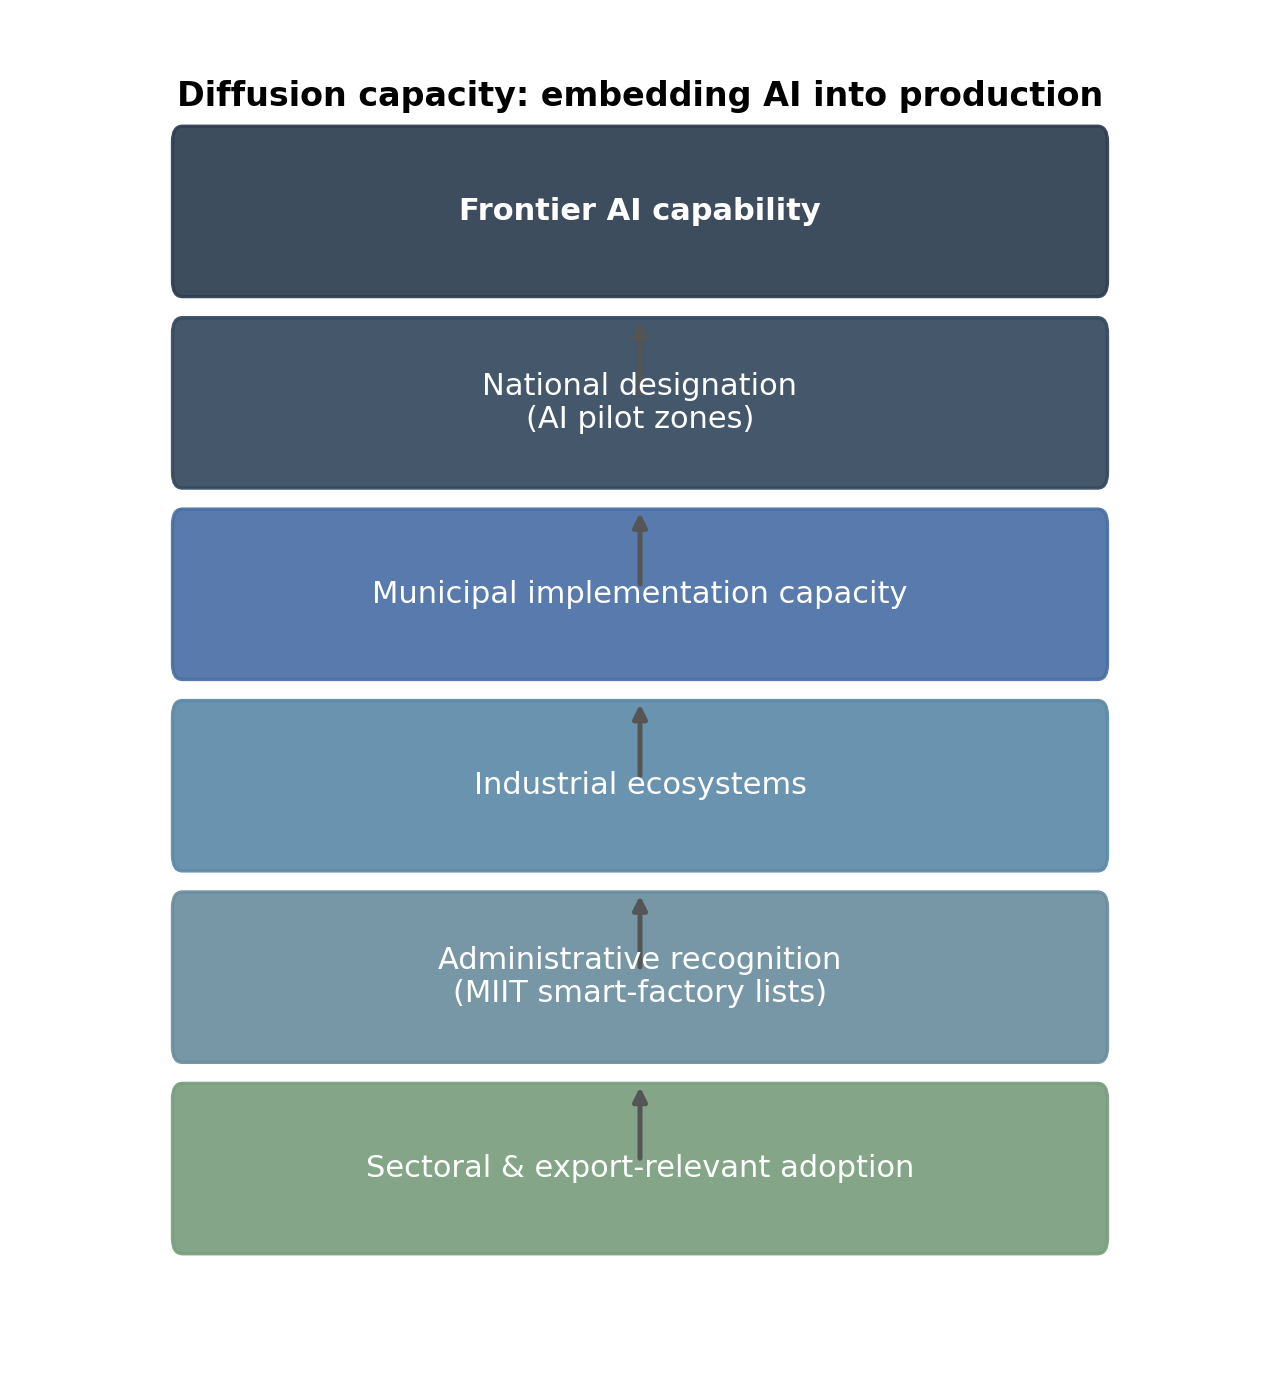
\includegraphics[width=0.92\linewidth]{paper/figures/fig_1_diffusion_state_architecture.png}
    \caption{Conceptual architecture of the AI diffusion state. The figure summarizes the paper's framework, moving from frontier AI capability to national designation, municipal implementation capacity, industrial ecosystems, administrative recognition, and sectoral and export-relevant industrial adoption.}
    \label{fig:diffusion_state_architecture}
\end{figure}

\begin{figure}[t]
    \centering
    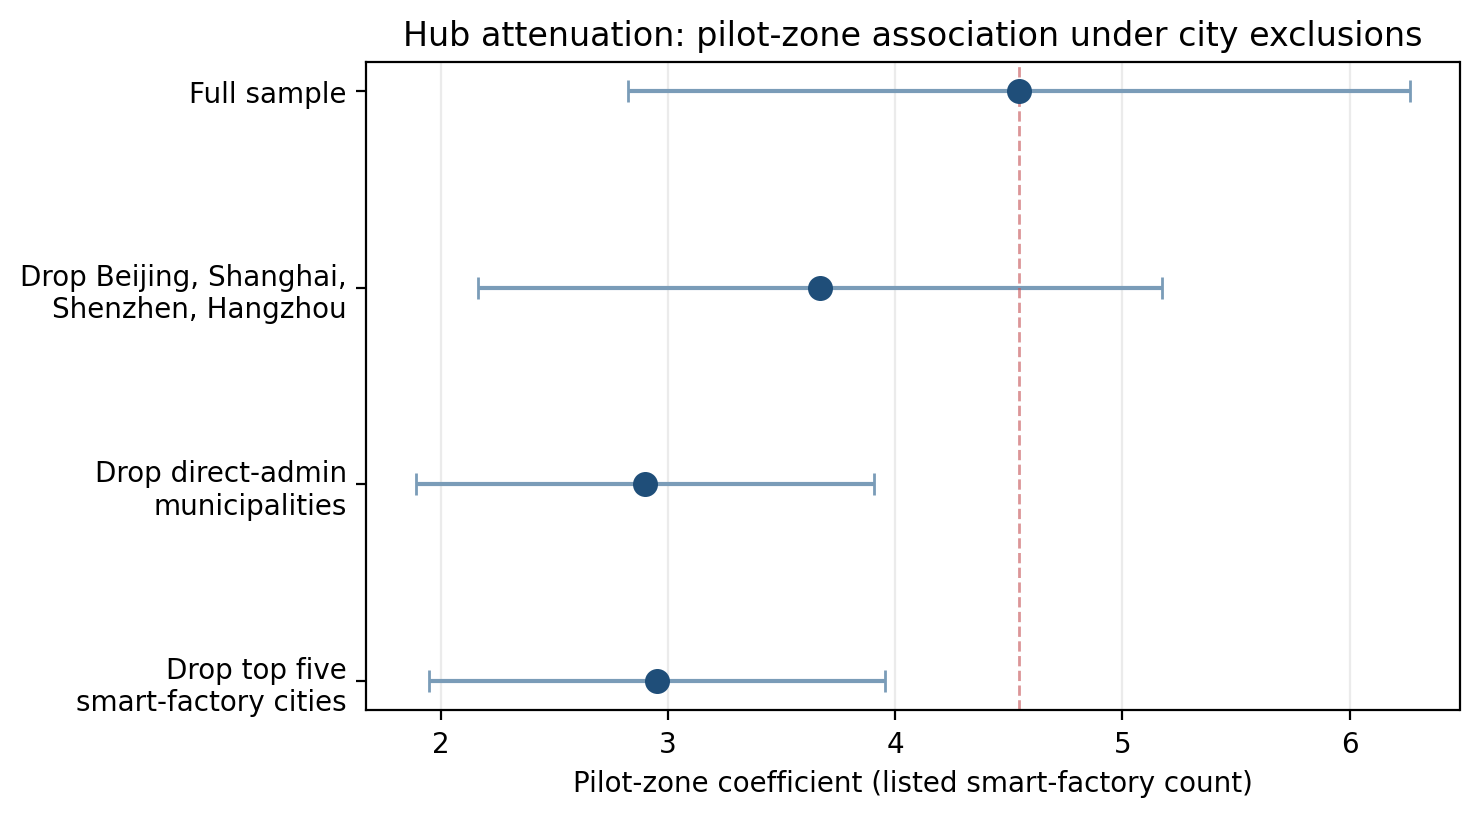
\includegraphics[width=0.92\linewidth]{paper/figures/fig_2_hub_attenuation_pilot_coefficients.png}
    \caption{Hub attenuation in the pilot-zone association. The figure plots the pilot-zone coefficient on listed smart-factory counts under the full sample and under hub-exclusion rules, with 95 percent confidence intervals. The attenuation pattern is interpreted as evidence of a hub-centered diffusion architecture rather than a uniform pilot-zone treatment effect.}
    \label{fig:hub_attenuation}
\end{figure}

\begin{figure}[t]
    \centering
    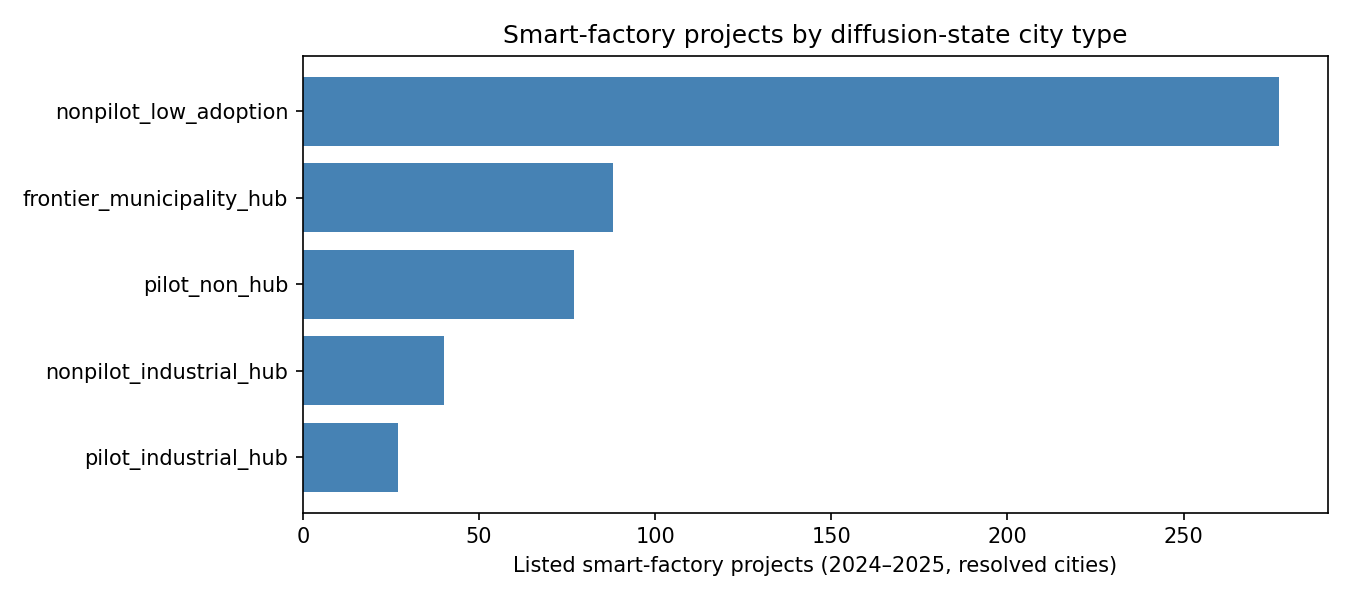
\includegraphics[width=0.92\linewidth]{paper/figures/fig_3_city_typology_smart_factory_counts.png}
    \caption{Listed smart-factory projects by ex ante diffusion-state city type. The figure shows how recognized adoption varies across city categories defined before using smart-factory outcomes, supporting the interpretation that adoption is organized through pilot status, administrative hierarchy, and industrial hub capacity.}
    \label{fig:city_typology}
\end{figure}

% -----------------------------
% Appendix figures
% -----------------------------

\begin{figure}[p]
    \centering
    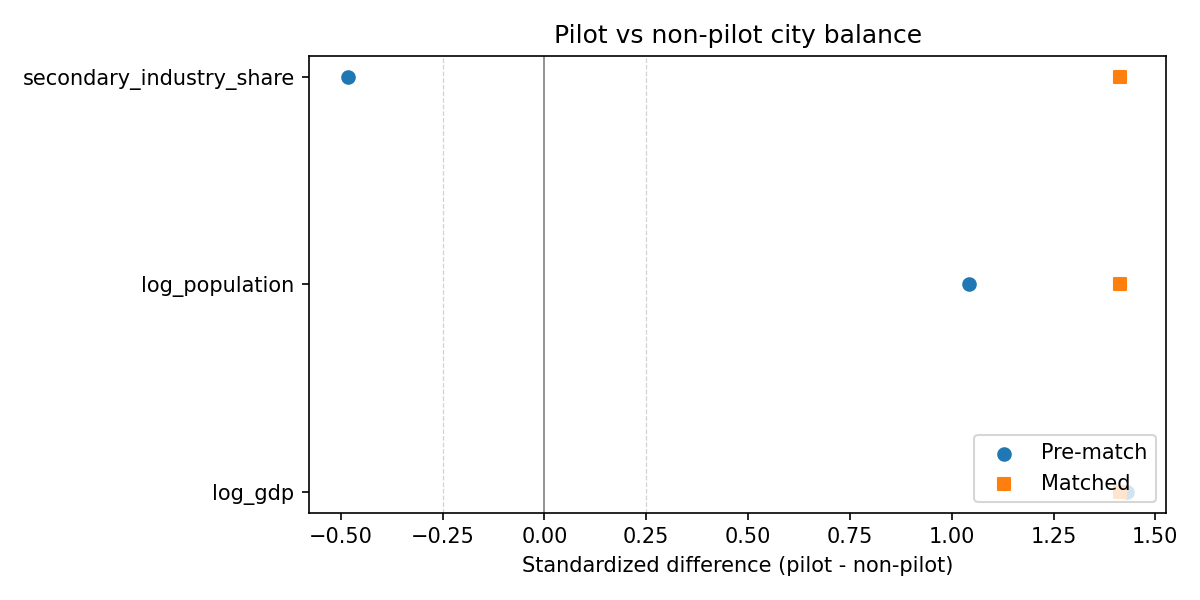
\includegraphics[width=0.92\linewidth]{paper/figures/fig_A1_balance_standardized_differences.png}
    \caption{Standardized mean differences for pilot and non-pilot cities. This appendix figure reports balance diagnostics for available city controls and should be interpreted as controls-dependent descriptive evidence.}
    \label{fig:balance_standardized_differences}
\end{figure}

\begin{figure}[p]
    \centering
    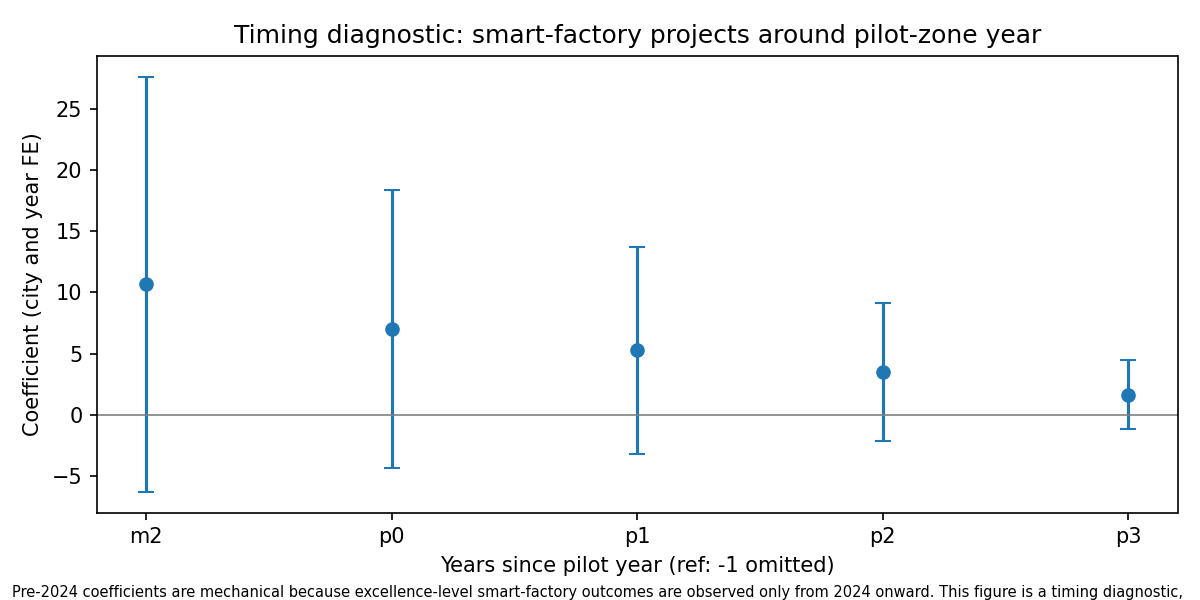
\includegraphics[width=0.92\linewidth]{paper/figures/fig_A2_timing_diagnostic_pilot_zones.png}
    \caption{Timing diagnostic for pilot-zone designation and listed smart-factory recognition. Pre-2024 smart-factory counts are zero-filled because public excellence-level lists begin in 2024, so the figure is a timing diagnostic rather than a pre-trend validation exercise.}
    \label{fig:timing_diagnostic}
\end{figure}
